\newpage % Rozdziały zaczynamy od nowej strony.
 

\section{Analiza przeprowadzonych eksperymentów}
\subsection{Architektury}
\begin{description}

\item[Zbadane architektury]
\hfill\\
\begin{table}[ht]
    \centering
    \resizebox{\textwidth}{!}{\begin{tabular}{cccclll}
        \hline
        \multicolumn{1}{|c|}{Długość sekwencji}   & \multicolumn{1}{c|}{Warstwa CNN}          & \multicolumn{1}{c|}{Liczba warstw LSTM} & \multicolumn{1}{c|}{Liczba neuronów w warstwie} & \multicolumn{1}{l|}{Top 1} & \multicolumn{1}{l|}{Top 5} & \multicolumn{1}{l|}{Top 10 z kolejnością} \\ \hline
        \multicolumn{1}{|c|}{1}                   & \multicolumn{1}{c|}{nie}                  & \multicolumn{1}{c|}{1}                  & \multicolumn{1}{c|}{512}                        & \multicolumn{1}{l|}{0.27}     & \multicolumn{1}{l|}{0.51}     & \multicolumn{1}{l|}{0.41}                    \\ \hline
        \multicolumn{1}{|c|}{\multirow{5}{*}{5}}  & \multicolumn{1}{c|}{\multirow{4}{*}{nie}} & \multicolumn{1}{c|}{\multirow{3}{*}{1}} & \multicolumn{1}{c|}{128}                        & \multicolumn{1}{l|}{0.23}     & \multicolumn{1}{l|}{0.59}     & \multicolumn{1}{l|}{0.37}                    \\ \cline{4-7} 
        \multicolumn{1}{|c|}{}                    & \multicolumn{1}{c|}{}                     & \multicolumn{1}{c|}{}                   & \multicolumn{1}{c|}{256}                        & \multicolumn{1}{l|}{0.16}     & \multicolumn{1}{l|}{0.42}     & \multicolumn{1}{l|}{0.27}                    \\ \cline{4-7} 
        \multicolumn{1}{|c|}{}                    & \multicolumn{1}{c|}{}                     & \multicolumn{1}{c|}{}                   & \multicolumn{1}{c|}{512}                        & \multicolumn{1}{l|}{0.30}     & \multicolumn{1}{l|}{0.63}     & \multicolumn{1}{l|}{0.43}                    \\ \cline{3-7} 
        \multicolumn{1}{|c|}{}                    & \multicolumn{1}{c|}{}                     & \multicolumn{1}{c|}{2}                  & \multicolumn{1}{c|}{128}                        & \multicolumn{1}{l|}{0.27}     & \multicolumn{1}{l|}{0.62}     & \multicolumn{1}{l|}{0.41}                    \\ \cline{2-7} 
        \multicolumn{1}{|c|}{}                    & \multicolumn{1}{c|}{tak}                  & \multicolumn{1}{c|}{1}                  & \multicolumn{1}{c|}{128}                        & \multicolumn{1}{l|}{0.24}     & \multicolumn{1}{l|}{0.53}     & \multicolumn{1}{l|}{0.36}                    \\ \hline
        \multicolumn{1}{|c|}{\multirow{5}{*}{10}} & \multicolumn{1}{c|}{\multirow{4}{*}{nie}} & \multicolumn{1}{c|}{\multirow{2}{*}{1}} & \multicolumn{1}{c|}{128}                        & \multicolumn{1}{l|}{0.06}     & \multicolumn{1}{l|}{0.25}     & \multicolumn{1}{l|}{0.13}                    \\ \cline{4-7} 
        \multicolumn{1}{|c|}{}                    & \multicolumn{1}{c|}{}                     & \multicolumn{1}{c|}{}                   & \multicolumn{1}{c|}{512}                        & \multicolumn{1}{l|}{0.13}     & \multicolumn{1}{l|}{0.45}     & \multicolumn{1}{l|}{0.26}                    \\ \cline{3-7} 
        \multicolumn{1}{|c|}{}                    & \multicolumn{1}{c|}{}                     & \multicolumn{1}{c|}{2}                  & \multicolumn{1}{c|}{128}                        & \multicolumn{1}{l|}{0.34}     & \multicolumn{1}{l|}{0.66}    & \multicolumn{1}{l|}{0.47}                    \\ \cline{3-7} 
        \multicolumn{1}{|c|}{}                    & \multicolumn{1}{c|}{}                     & \multicolumn{1}{c|}{2}                  & \multicolumn{1}{c|}{512}                        & \multicolumn{1}{l|}{0.12}     & \multicolumn{1}{l|}{0.44}     & \multicolumn{1}{l|}{0.24}                    \\ \cline{2-7} 
        \multicolumn{1}{|c|}{}                    & \multicolumn{1}{c|}{tak}                  & \multicolumn{1}{c|}{1}                  & \multicolumn{1}{c|}{128}                        & \multicolumn{1}{l|}{0.17}     & \multicolumn{1}{l|}{0.56}     & \multicolumn{1}{l|}{0.32}                    \\ \hline
        \multicolumn{1}{|c|}{\multirow{2}{*}{15}} & \multicolumn{1}{c|}{\multirow{2}{*}{nie}} & \multicolumn{1}{c|}{\multirow{2}{*}{1}} & \multicolumn{1}{c|}{128}                        & \multicolumn{1}{l|}{0.03}     & \multicolumn{1}{l|}{0.10}     & \multicolumn{1}{l|}{0.06}                    \\ \cline{4-7} 
        \multicolumn{1}{|c|}{}                    & \multicolumn{1}{c|}{}                     & \multicolumn{1}{c|}{}                   & \multicolumn{1}{c|}{512}                        & \multicolumn{1}{l|}{0.10}     & \multicolumn{1}{l|}{0.38}     & \multicolumn{1}{l|}{0.21}                    \\ \hline
                                                  &                                           &                                         &                                                 &                            &                            &                                          
        \end{tabular}}
    \caption{Uzyskane skuteczności w eksperymentach} 
    \label{wyniki}
\end{table} 

\item[Wyróżniona architektura]
\hfill\\
\label{wyrozniony}
Ze wstępnych badań najlepsze wyniki uzyskał model o parametrach przedstawionych w tabeli \ref{parametry wstepne}. 
\begin{table}[ht]
    \centering
    \begin{tabular}{|l|l|}
        \hline
        \multicolumn{1}{|c|}{parametr} & wartość   \\ \hline
        liczba warstw rnn              & 2                 \\ \hline
        rodzaj rnn                     & lstm              \\ \hline
        liczba neuronów w warstwie     & 128               \\ \hline
        długość sekwencji wejściowej   & 10                \\ \hline
        liczba trenowanych parametrów  & 3,434,177         \\ \hline
        rozmiar słownika               & 20000             \\ \hline
        rozmiar wektora zanurzeń       & 32                \\ \hline
        rozmiar porcji danych          & 128               \\ \hline
        liczba epok                    & 25                \\ \hline
        optymalizator                  & adam              \\ \hline
        funkcja celu                   & entropia krzyżowa \\ \hline
        \end{tabular}
    \caption{Parametry najlepszego modelu z badań wstępnych} 

    \label{parametry wstepne}
\end{table} \\\\\\\\\\\\\\\\\\\\\\
Uzyskując skuteczności przedstawione w tabeli \ref{wyniki_najlepszego}. 
\begin{table}[ht]
    \centering
    \begin{tabular}{|l|l|}
        \hline
        \multicolumn{1}{|c|}{Miara}  & Wynik\\ \hline
        Top 1                            & 0.34  \\ \hline
        Top 3                            & 0.56  \\ \hline
        Top 5                            & 0.66  \\ \hline
        Top 5 z kolejnością              & 0.46  \\ \hline
        Top 10 z kolejnością             & 0.47  \\ \hline
        najmniejsza wartość funkcji celu & 1.67  \\ \hline
        \end{tabular}
    \caption{Wyniki uzyskane przez najlepszy model z badań wstępnych} 

    \label{wyniki_najlepszego}
\end{table} \\
Model ten osiągnął znacznie lepsze wyniki niż pozostałe badane modele. Na tym modelu zostaną wykonane dalsze badania 
dotyczące większego rozmiaru słownika oraz zastosowania warstwy gru zamiast lstm. 
\end{description}
\subsection{Różne rozmiary słownika}
Kolejnym etapem badań jest sprawdzenie jak zachowa się model przy większych rozmiarach słownika. Przy badańach wstępnych 
wynosiła ona \begin{math}20000\end{math}. W tym eksperymencie użyje rozmiaru słownika takiego samego jak użyli w 
swojej pracy autorzy \cite{hellendoorn} wynoszącego 74000. Dla takiego rozmiaru pomijane są słowa 
występujące rzadziej niż 5 razy. wszystkie pozostałe parametry pozostają takie same.
\begin{table}[ht]
    \centering
    \begin{tabular}{|l|l|}
        \hline
        \multicolumn{1}{|c|}{Miara}  & Wynik\\ \hline
        Top 1                            & 0.30 \\ \hline
        Top 3                            & 0.52 \\ \hline
        Top 5                            & 0.61 \\ \hline
        Top 5 z kolejnością              & 0.42 \\ \hline
        Top 10 z kolejnością             & 0.43 \\ \hline
        najmniejsza wartość funkcji celu & 1.75 \\ \hline
        \end{tabular}
    \caption{Wyniki uzyskane przez model o dużym słowniku} 
    \label{wyniki_duzego}

\end{table} \\ 

\subsection{Zastosowanie warstwy gru}
Ostatnim wykonanym przeze mnie eksperymentem jest porównanie skuteczności warstwy gru z warstwą lstm. Badanie to przeprowadzam 
dla parametrów wyróżnionego modelu \ref{wyrozniony} podmieniając rodzaj warstwy rnn. Uzyskane wyniki zostały przedstawione w tabeli \ref{wyniki_gru}. 
\begin{table}[ht]
    \centering
    \begin{tabular}{|l|l|}
        \hline
        \multicolumn{1}{|c|}{Miara}  & Wynik\\ \hline
        Top 1                            & 0.32 \\ \hline
        Top 3                            & 0.59 \\ \hline
        Top 5                            & 0.68 \\ \hline
        Top 5 z kolejnością              & 0.46 \\ \hline
        Top 10 z kolejnością             & 0.47 \\ \hline
        najmniejsza wartość funkcji celu & 1.57 \\ \hline
        \end{tabular}
    \caption{Wyniki uzyskane przez model o warstwie GRU} 

    \label{wyniki_gru}
\end{table} \\ 

\subsection{przegląd hiperparametrów}
\begin{description}
    \item[Wpływ długości sekwencji wejściowe] 
    \hfill \\ Model został wytrenowany na czterech długościach sekwencji wejściowej: \begin{math}1, 5, 10, 15\end{math}. Można
    zaobserwować wzrost skuteczności modelu wraz ze wzrostem sekwencji, do 10 słów. dalsze próby powiększania sekwencji wpływają negatywnie 
    na jego działanie. spowodowane jest to tym, że dla krótkich sekwencji takich jak \begin{math}1, 5\end{math} model posiada za mało 
    kontekstu aby wykonać predykcję, natomiast sekwencje długości 15 są już zbyt specyficznymi częściami konkretnego programu aby móc je 
    uogólnić dla przewidywanego kodu. \\
    \item[Wpływ długości rozmiaru słownika] 
    \hfill \\ Wielkość słownika ma duży wpływ na działanie modelu. Przy małych wielkościach można spodziewać się niepoprawnego działania 
    ze względu na to, że sieć nie będzie znała słów, które ma przewidywać. 
    jak pokazują wyniki eksperymentu w tabeli \ref{wyniki_duzego}, słownik o bardzo dużej liczbie słów również pogarsza działanie algorytmu. 
    Różnica ta wynosi około \begin{math}5 \end{math} punktów procentowych we wszystkich kategoriach. Duże rozmiary słownika również znaczenie spowalniają 
    proces treningu. \\
    \item[Liczba warstw sieci rekurencyjnej]
    \hfill \\ Eksperymenty zostały przeprowadzone dla jednej oraz dwóch warstw sieci rekurencyjnej. 
    We wszystkich przeprowadzonych eksperymentach, modele o dwóch warstwach osiągnęły podobne lub lepsze wyniki od modeli o jednej warstwie. \\
    \item[Wpływ liczby neruronów w warstwie rekurencyjnej]
    \hfill \\ Eksperymenty zostały przeprowadzone dla warstw składających cie z \begin{math} \end{math} warstw sieci rekurencyjnej. Można 
    zaobserwować, że duże liczby neuronów w warstwie nie poprawiają działania modelu. Najlepszy rezultat oraz inne rezultaty zbliżone 
    do niego uzyskują warstwy składające się ze 128 neuronów. \\
    \item[Wpływ warstwy CNN]
    \hfill \\ Przeprowadziłem dwa eksperymenty z zastosowaniem warstwy CNN, oba dla jednej warstwy LSTM o 128 neuronach różniących się długością 
    sekwencji wejściowe. Po porównaniu tych modeli z modelami o tych samych parametrach bez warstwy CNN, zauważalna jest nieznaczna poprawa, około 
    \begin{math}1\end{math} punkt procentowy dla modelu o długości sekwencji równej \begin{math}5\end{math}, oraz około \begin{math}10\end{math} 
    punktów procentowych dla modelu o długości wejściowej równej 10. Mimo poprawy modele te wciąż osiągają znacznie gorsze wyniki od 
    pozostałych badanych modeli. \\
    \item[Zastosowanie warstwy GRU]
    \hfill \\ Zastosowanie warstwy GRU poprawiło działanie wyróżnionego modelu w kategoriach Top 3 oraz Top 5, natomiast pogorszyło w Top 1. Różnice te są jednak bardzo 
    niewielkie, wynoszą około \begin{math}2 \end{math} punktów procentowych i najprawdopodobniej wynikają z losowości procesu uczenia. Można 
    wywnioskować zatem, że w tak przedstawionym zadaniu rodzaj zastosowanej warstwy nie ma wpływu na skuteczność modelu. Warto zatem użyć warstwy 
    GRU w celu skrócenia czasu treningu. \\
  \end{description}

\subsection{Najlepsza znaleziona architektura}
  Jako, że model trenowany jest z myślą o stworzeniu wtyczki ułatwiającej pisanie kodu, do wybrania najlepszej architektury posłużę się 
  metryką uwzględniającą 5 najlepszych podpowiedzi z uwzględnieniem kolejności wystąpienia. W tym kryterium oba modele scharakteryzowane 
  w sekcjach \ref{wyniki_gru}, \ref{wyniki_najlepszego} uzyskują taką samą skuteczność wynoszącą \begin{math}46\%\end{math}, jednak dla 
  5 najlepszych parametrów bez uwzględnia kolejności radzi sobie lepiej model przedstawiony w \ref{wyniki_gru} osiągając skuteczność 
  równą \begin{math}68\%\end{math}, zatem to on zostanie 
  użyty w implementacji wtyczki oraz porównania z architekturami z innych prac. W tabeli \ref{najelpszy} przedstawiam dokładne parametry tego modelu. 
  \begin{table}[ht]
    \centering
    \begin{tabular}{|l|l|}
        \hline
        \multicolumn{1}{|c|}{parametr} & wartość           \\ \hline
        liczba warstw rnn              & 2                 \\ \hline
        rodzaj rnn                     & GRU                \\ \hline
        liczba neuronów w warstwie     & 128               \\ \hline
        długość sekwencji wejściowej   & 10                \\ \hline
        liczba trenowanych parametrów  & 3,434,177         \\ \hline
        rozmiar słownika               & 20000             \\ \hline
        rozmiar wektora zanurzeń       & 32                \\ \hline
        rozmiar porcji danych          & 128               \\ \hline
        liczba epok                    & 25                \\ \hline
        optymalizator                  & adam              \\ \hline
        funkcja celu                   & entropia krzyżowa \\ \hline
        \end{tabular}
    \caption{Wybrany najlepszy model} 

    \label{najelpszy}
\end{table} 

Na wykresie \ref{wykres} została przedstawiona wartość funkcji celu w kolejnych epokach treningu. 
\begin{figure}[!h]
	% Znacznik \caption oprócz podpisu służy również do wygenerowania numeru obrazka;
    \caption{Wartość funkcji celu w kolejnych epokach}

	% dlatego zawsze pamiętaj używać najpierw \caption, a potem \label
    \label{wykres}
    % Zamiast width można też użyć height, etc. 
    \centering 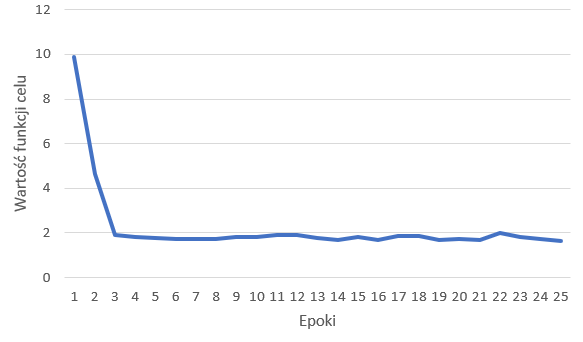
\includegraphics[width=103mm, height=76mm]{wykres.png}
\end{figure}

\subsection{Generowane wyniki}
\begin{figure}[!h]
	% Znacznik \caption oprócz podpisu służy również do wygenerowania numeru obrazka;
    \caption{Przykładowy wynik wygenerowany przez model}

	% dlatego zawsze pamiętaj używać najpierw \caption, a potem \label
    \label{fig:wynik}
    % Zamiast width można też użyć height, etc. 
    \centering 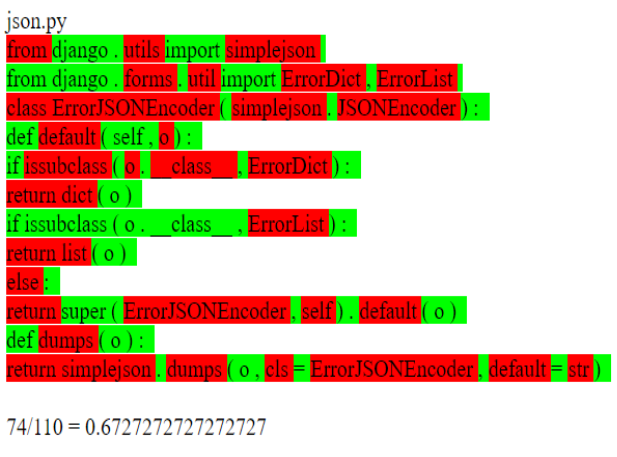
\includegraphics[width=103mm, height=76mm]{wynik.png}
\end{figure}
Na rysunku \ref{fig:wynik} został przedstawiony przykładowy program którego uzupełnienie realizował model. Na zielono zostały zaznaczone tokeny,
które znalazły się w 5 pierwszych predykcjach modelu, pozostałe tokeny oznaczone zostały kolorem czerwonym. Można zaobserwować, że 
model w bardzo dobrym stopniu radzi sobie z przewidywaniem struktury programu, uzupełnianiem nawiasów, wykrywaniem końca linii, stawianiem słów kluczowych. 
Gorzej radzi sobie z uzupełnianiem nazw pochodzących z bibliotek oraz definiowanych zmiennych. 

\subsection{Porównanie uzyskanych wyników}
Modele pochodzące z przytoczonych prac pełnią to samo zadanie, jednak trenowane są na innych zbiorach danych. Mimo to, 
uzyskany przeze mnie model osiąga bardzo zbliżone do nich wyniki, oraz warto zestawić je ze sobą. 

Autor \cite{erik} uzyskał model o skuteczności wynoszącej \begin{math}69.7\%\end{math}, dla 
5 najlepszych wyników. Jest to niemal identyczny wynik z modelem uzyskanym przeze mnie. Mimo to architektury 
modeli znacznie różnią się, gdyż w pracy zastosował jedną warstwę LSTM o 512 neuronach. Różnica ta może wynikać z narzucenia innych 
hiperparametrów. 

Autor \cite{contextual_code_completion} uzyskał model o skuteczności wynoszącej \begin{math}66.3\%\end{math} dla 3 najlepszych predykcji, bez uwzględniania 
kolejności ich wystąpienia. Skuteczność mojego modelu w tej kategorii jest mniejsza, gdyż wynosi ona \begin{math}0.59\%\end{math}. Różnica 
ta najprawdopodobniej wynika z tego, że model przedstawiony w pracy \cite{contextual_code_completion} jest trenowany oraz testowany na pojedyńczych bibliotekach, 
zatem realizuje on znacznie prostsze zadanie. Modele te również wykorzystują całkowicie inną architekturę. Wykorzystany zostaje model ze skupieniem uwagi składający 
się z 3 nieliniowych warstw. 

W pracy autorzy \cite{hellendoorn} uzyskują model o skuteczności wynoszącej \begin{math}67.9\%\end{math}, dla 10 najlepszych predykcji z uwzględnieniem 
kolejności ich wystąpienia. Mój model osiąga w tej metryce gorszy wynik, równy \begin{math}47\%\end{math}. Różnice te mogą wynikać z znacznie 
dłuższego czasu treningu wynoszącego około 3 dni, oraz z bardziej złożonego mechanizmu predykcji, uwzględniającego zagnieżdżenia w kodzie. 

\subsection{Możliwe błędy}
Wszystkie oceniane przeze mnie modele trenowane były tylko raz. Ze względu na długi czas wykonania pojedyńczego eksperymentu, zdecydowałem 
się na porównanie ze sobą wiele różnych modeli zamiast kilku modeli kilkakrotnie trenowanych. Efektem tego mogą być nieprecyzyjne wyniki 
wynikające z losowości procesu uczenia, gdyż rozmiar próbki równy 1, jest zdecydowanie za mały aby dokładnie określić działanie modelu. 
Jako, że nie posiadamy jeszcze wystarczającej wiedzy na temat cech wspólnych pomiędzy językami programowania a językami naturalnymi, 
sugerowanie się modelami pochodzącymi z tej dziedziny nie przynosi odpowiednich rezultatów. 

Wszystkie zastosowane miary traktują przewidziane tokeny równo. Nie oddają one zatem dokładnie w jakim stopniu wtyczka usprawnia pracę 
programisty, gdyż przewidzenie długiej nazwy oszczędza znacznie więcej czasu niż np. pojedyńczego przecinka. 

Relacja pomiędzy kryteriami, którymi są oceniane modele, a faktyczną skutecznością tych modeli w praktyce jest nie znana. Zbyt duża liczba 
sugestii proponowanych przez model również negatywnie wpływa na pracę programisty, ponieważ sprawia, że pole zawierające sugestie staje 
się nieczytelne. Ocena z uwzględnieniem kolejności zakłada, że predykcja znajdująca się na drugim miejscu jest tylko w połowie tak użyteczna, 
jak ta znajdująca się na miejscu pierwszym, natomiast sugestia na trzecim miejscu tylko w jednej trzeciej itd. Założenie to wynika z tego, że 
wybranie niższej oceny wymaga więcej pracy od programisty. Mimo to łatwo pominąć ten problem np. stosując skróty klawiszowe, zatem 
nie jesteśmy w stanie określić, czy to założenie jest poprawne. 





